 
\section{Programa}

\begin{figure}
\centering
% Define block styles
\tikzstyle{decision} = [diamond, draw, fill=blue!20, 
    text width=4.5em, text badly centered, node distance=4cm, inner sep=0pt]
\tikzstyle{block} = [rectangle, draw, fill=blue!20, 
    text width=6em, text centered, rounded corners, minimum height=4em]
\tikzstyle{line} = [draw, -latex', ultra thick]
\tikzstyle{cloud} = [draw, ellipse,fill=red!20, node distance=3cm,
    minimum height=2em]
    
\begin{tikzpicture}[node distance = 4cm, auto]
    % Place nodes
    \node [block] (init) {Simuliacijos būsenos išsaugojimas};
    \node [block, below of=init] (timestep) {\( t_j = t_{j-1} + \Delta t_j\)};
    \node [block, below of=timestep] (calculate) {Naujos būsenos skaičiavimai};
    \node [block, left of=timestep] (change) {\(\Delta t_j = \frac{\Delta t_j}{10}\)};
    \node [block, left of=calculate] (restore) {Atstatome paskutinę sistemos būseną};
    \node [decision, below of=calculate] (check) {Ar pažeisti tikslumo reikalavimai?};
    \node [decision, right of=check, node distance=8cm] (end) {Ar simuliacija baigta?};
    \node [decision, above of=end] (timecheck) {Ar galima atstatyti laiko žingsnį?};
    \node [block, right of=timestep] (backroll) {\(\Delta t_j = 10 \Delta t_j \)};
    \node [block, below of=end] (final) {Pabaiga};

    % Draw edges
    \path [line] (init) -- (timestep);
    \path [line] (timestep) -- (calculate);
    \path [line] (calculate) -- (check);
    \path [line] (check) -| node [near start] {Taip} (restore);
    \path [line] (restore) -- (change);
    \path [line] (change) |- (init);
    \path [line] (check) -- node [near start] {Ne} (end);
    \path [line] (end) -- node [near start] {Ne} (timecheck);
    \path [line] (timecheck) |- node [near start] {Ne} (init);
    \path [line] (timecheck) -- node [near start] {Taip} (backroll);
    \path [line] (backroll) -- (init);
    \path [line] (end) -- node [near start] {Taip} (final);
\end{tikzpicture}
\caption{Algoritmo veikimas}
  \label{fig:algoritmas}
\end{figure}

Krūvininkų pernašos reiškiniai skaitmeniškai modeliuojami jau gana seniai \cite{juška:4946}, tam yra parašyta nemažai programų, tačiau daugelis jų yra pritaikytos vienai medžiagų klasei arba vienam eksperimento variantui. Tuo tarpu šiame darbe aptariama programa rašyta norint kuo plačiau ją taikyti, darant kuo mažesnius pakeitimus išeities tekste. Dėl to remtasi objektinio programavimo paradigma, skaidant programos funkcijas į atskirus elementus, kurie veikia nepriklausomai vienas nuo kito ir suteikia vartotojui galimybę keisti programos funkcionalumą nekeičiant pačios programos.
\subsection{Veikimas}

\begin{wrapfigure}{r}{0.5\textwidth}
  \begin{center}
	% Define block styles
\tikzstyle{block} = [rectangle, draw, fill=blue!20, 
    text width=10em, text centered, rounded corners, minimum height=4em]
\tikzstyle{line} = [draw, -latex', ultra thick]
\tikzstyle{cloud} = [draw, ellipse,fill=red!20, node distance=3cm,
    minimum height=4em]
    
\begin{tikzpicture}[node distance = 3cm, auto]
    % Place nodes
	\node [block] (field) {Suskaičiuojamas momentinis elektrinio lauko pasiskirstymas bandinyje};    
    \node [block, below of=field] (recom) {Suskaičiuojami rekombinavę krūvininkai};
    \node [block, below of=recom] (car) {Suskaičiuojami dreifuojantys ir difunduojantys krūvininkai};
    \node [block, below of=car] (sum) {Susumuojamas srovės tankis};

    % Draw edges
    \path [line] (field) -- (recom);
    \path [line] (recom) -- (car);
    \path [line] (car) -- (sum);
\end{tikzpicture}
  \end{center}
  \caption{Skaičiavimo seka}
  \label{fig:skaičiavimas}
\end{wrapfigure}

Programa veikia remdamasi įvesties failu, kuriame yra apibūdintas simuliuojamas eksperimentas, surašomi fizikiniai parametrai ir pasirenkamos pradinės sąlygos. Pagrindinis programos ciklas skaito ir atpažįsta komandas įvesties faile, bei iškviečia atitinkamus programos modulius toms komandoms įvykdyti. Šios programos patogumą padidina ir integruotas skaičiuotuvo modulis, leidžiantis įvesties faile atlikti daugelį matematinių veiksmų, taip palengvinant teorinio modelio sutapatinimą su atliekamu eksperimentu.
Visoje programoje naudojami nenormuoti fizikiniai dydžiai SI sistemos vienetais.
\subsection{Moduliai}
Programai sukurti keli atskiri moduliai, kurie leidžia ją taikyti įvairių eksperimentų teoriniams rezultatams modeliuoti, tarkime lėkio trukmės matavimams (ToF). Šiame darbe naudoti moduliai yra skirti photo-CELIV skaičiavimams. Kiekvienas iš anksčiau paminėtų modulių naudojasi baziniu moduliu, kuris skirtas tankio pasiskirstymo uždavinių sprendimui. Jo veikimo schema pavaizduota  \ref{fig:algoritmas} paveiksliuke. Šiame modulyje veikia adaptyvaus laiko žingsnio algoritmas, kuris leidžia didinti ir mažinti laiko žingsnį priklausomai nuo skaičiavimų tikslumo sąlygos \eqref{eq:tikslumas}. Bazinis modulis savo ruožtu naudoja skaičiavimo modulį atskiriems fizikiniams reiškiniams įtraukti. Toks programos skaidymas leidžia nesunkiai modifikuoti programos darbą įjungiant arba išjungiant atskirus fizikinių skaičiavimų modulius. Tačiau fizikinių reiškinių įtraukimo seka yra griežtai nurodyta (žr.  \ref{fig:skaičiavimas} pav.).

Visiems fizikiniams skaičiavimams reikia vieną kartą „pereiti“ per visą bandinio sudalinimų masyvą, atliekant skaičiavimus su kiekvienu narveliu atskirai. Dėl to visų fizikinių skaičiavimų sudėtingumas yra \(\sim O(M)\). Akivaizdu, jog suminis visos simuliacijos sudėtingumas yra \(O(M \cdot K)\), kur \(K\) atliktų laiko iteracijų skaičius. Laiko žingsnio parinkimas patikimas programos vykdymo metu veikiančiam algoritmui, kuris seka, ar nepažeidžiami tikslumo reikalavimai:
\begin{equation} \label{eq:tikslumas}
\begin{array}{c}
\Delta N_{i,j+1} < \alpha N_{i,j} \\
\Delta P_{i,j+1} < \alpha P_{i,j}
\end{array}
\end{equation}
Algoritmas stebi judančių ir rekombinuojančių krūvininkų kiekius ir tikrina ar jie neviršija nustatytos maksimalios narvelyje esančių krūvininkų dalies \(\alpha\). Viršijus pastarąją vertę laiko žingsnis mažinamas, o paskutinis simuliacijos žingsnis kartojamas iš naujo. Papildoma funkcija, kurią atlieka algoritmas yra laiko žingsnio didinimas. Todėl kas 100 žingsnių algoritmas aklai padidina laiko žingsnį ir stebi ar nepažeidžiama tikslumo sąlyga.
Geriausiu atveju \(K= \frac{t_{simuliacijos}}{\Delta t_{maksimalus}}\), blogiausiu atveju \(\Delta t \rightarrow 0 \) ir simuliacija nustoja veikti, pasiūlydama vartotojui pakeisti erdvinį sudalinimą. \( \Delta t_{maksimalus} \) yra parenkamas įvesties faile.

Jei skaičiavimuose reikalinga aproksimacija, visur be išimčių naudojami tiesiniai artiniai, dėl to tikslumas priklauso nuo sudalinimų skaičiaus \(M\) pirmame laipsnyje.

\subsection{Simuliacija}

\begin{figure}
\centering
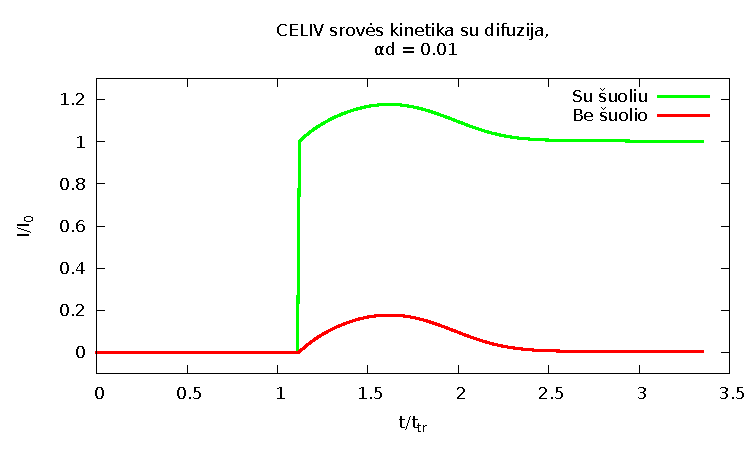
\includegraphics[width=\textwidth]{./media/pdf/jump.pdf} 
\caption{CELIV kinetikos be talpinio šuolio ir su juo}
\label{fig:suoliai}
\end{figure}


Šios programos funkcija -- atkartoti realaus eksperimento eigą ir pateikti teorinį rezultatą, kurį galima tapatinti su realiu eksperimentu.

Realios photo-CELIV kinetikos susideda iš dviejų dalių: talpinio šuoliuko, atsirandančio dėl išorinės įtampos, prijungtos prie bandinio, ir krūvininkų ištraukimo sąlygotos kinetikos dalies \cite{juška:4946}. Šioje programoje dėl paprastumo talpinis šuoliukas nėra modeliuojamas (žr. \ref{fig:suoliai}~pav.). Jis pridedamas apdorojimo metu \(I_0 = \frac{\varepsilon \varepsilon_0 A S}{d}\).

Kinetikos atvaizduojant normuotos į srovę \(I_0\) ir į teorinę CELIV lėkio trukmę \(t_{tr} = d \sqrt{\frac{2}{\mu A}} \) \cite{juška:155202}. Čia \(A\) [CELIV] įtampos kilimo koeficientas.

Norėdami ištirti difuzijos įtaką krūvininkų pernašai photo-CELIV atveju simuliuojame eksperimentą, kurio metu po fotogeneracijos bandinys paliekamas laikui \(t_{delay}\) atjungtas nuo išorinės grandinės, taigi jo viduje vyksta tik krūvininkų rekombinacija ir difuzija. Tokiu būdu galime atskirti stiprų pradinį difuzijos signalą nuo kitos CELIV signalo dalies.

Norėdami ištirti difuzijos įtaką krūvininkų rekombinacijos spartos matavimui, simuliuojame realų rekombinacijos spartos matavimą: keičiame \(t_{delay}\) ir sekame photo-CELIV srovės maksimumo vertės kitimą. Iš sumodeliuotų maksimumo vertės priklausomybių nuo užlaikymo trukmės galėsime nustatyti atsirandančią paklaidą dėl difuzijos.

\subparagraph*{Papildomos sąlygos,}\label{page:params} kurių laikėmės visų modeliavimų metu: Trikampio įtampos signalo trukmė 0.1ms, įtampa kinta nuo 0 iki 1V. Krūvininkų judrių santykis \(\frac{\mu_n}{\mu_p} = 1000\), taigi praktiškai juda tik vieni krūvininkai, mūsų atveju -- su neigiamu krūviu. Pasirinkti pilnai blokuojantys bandinio kontaktai, tokie, kad krūvininkai per juos negalėtų nei patekti į bandinį  nei išeiti iš jo.
Pasirinktas fotogeneracijos intensyvumo parametras \(I_0 S \equiv L = 10^6 \) nes su tokia verte daugelyje kinetikų pasiekiama soties nuo generacijos intensyvumo vertė, plačiau aprašyta \cite{juška:155202}. Pavyzdinis tokios simuliacijos įvesties failas pateiktas priede \ref{app:failas}.